\chapter{Síntese de controladores}    \label{chp:sintese}
    \section{Metodologia}
    
	\section{Sistema de Tração - Controle de velocidade tangencial}
	
	    \begin{equation}
	        G_T(s) = \frac{c_1}{s + c_2}
	    \end{equation}
	    
	    \begin{equation}
	        C_T(s) = K_p + \frac{K_i}{s} = \frac{K_p s + K_i}{s}
	    \end{equation}
	    
	    \begin{equation}
	        M_{AT}(s) = G_T(s) C_T(s) = \frac{c_1 K_p s + c_1 K_1}{s (s + c_2}
	    \end{equation}
	    
	    \begin{equation}
	        M_{FT} = \frac{c_1 K_p s + c_1 K_i}{s^2 + (K_p c_1 + c_2) s + c_1 K_i}
	    \end{equation}
	    
	    A função de transferência desejada para malha fechada tem que obrigatoriamente possuir o mesmo zero 
	    
	    \begin{equation}
	        D(s) = \frac{c_1 K_p s + \omega_n^2}{s^2 + 2 \zeta \omega_n s + \omega_n^2}
	    \end{equation}
	    
	    $M_{FT}(s) = D(s)$
	    
	    \begin{equation}
	        \left\{
	        \begin{array}{cc}
    	        K_p c_1 + c_2 = 2 \zeta \omega_n \\
    	        K_i c_1 = \omega_n^2
    	   \end{array}\right
	    \end{equation}
	    
	    \begin{equation}
	        \left\{
	        \begin{array}{cc}
    	        K_p = \frac{2 \zeta \omega_n - c_2}{c_1} \\
    	        K_i = \frac{\omega_n^2}{c_1}
    	    \end{array}\right
	    \end{equation}
	    
	    \subsection{Dinâmica de Saturação}
	    
	        \begin{figure}[h]
                \centering
                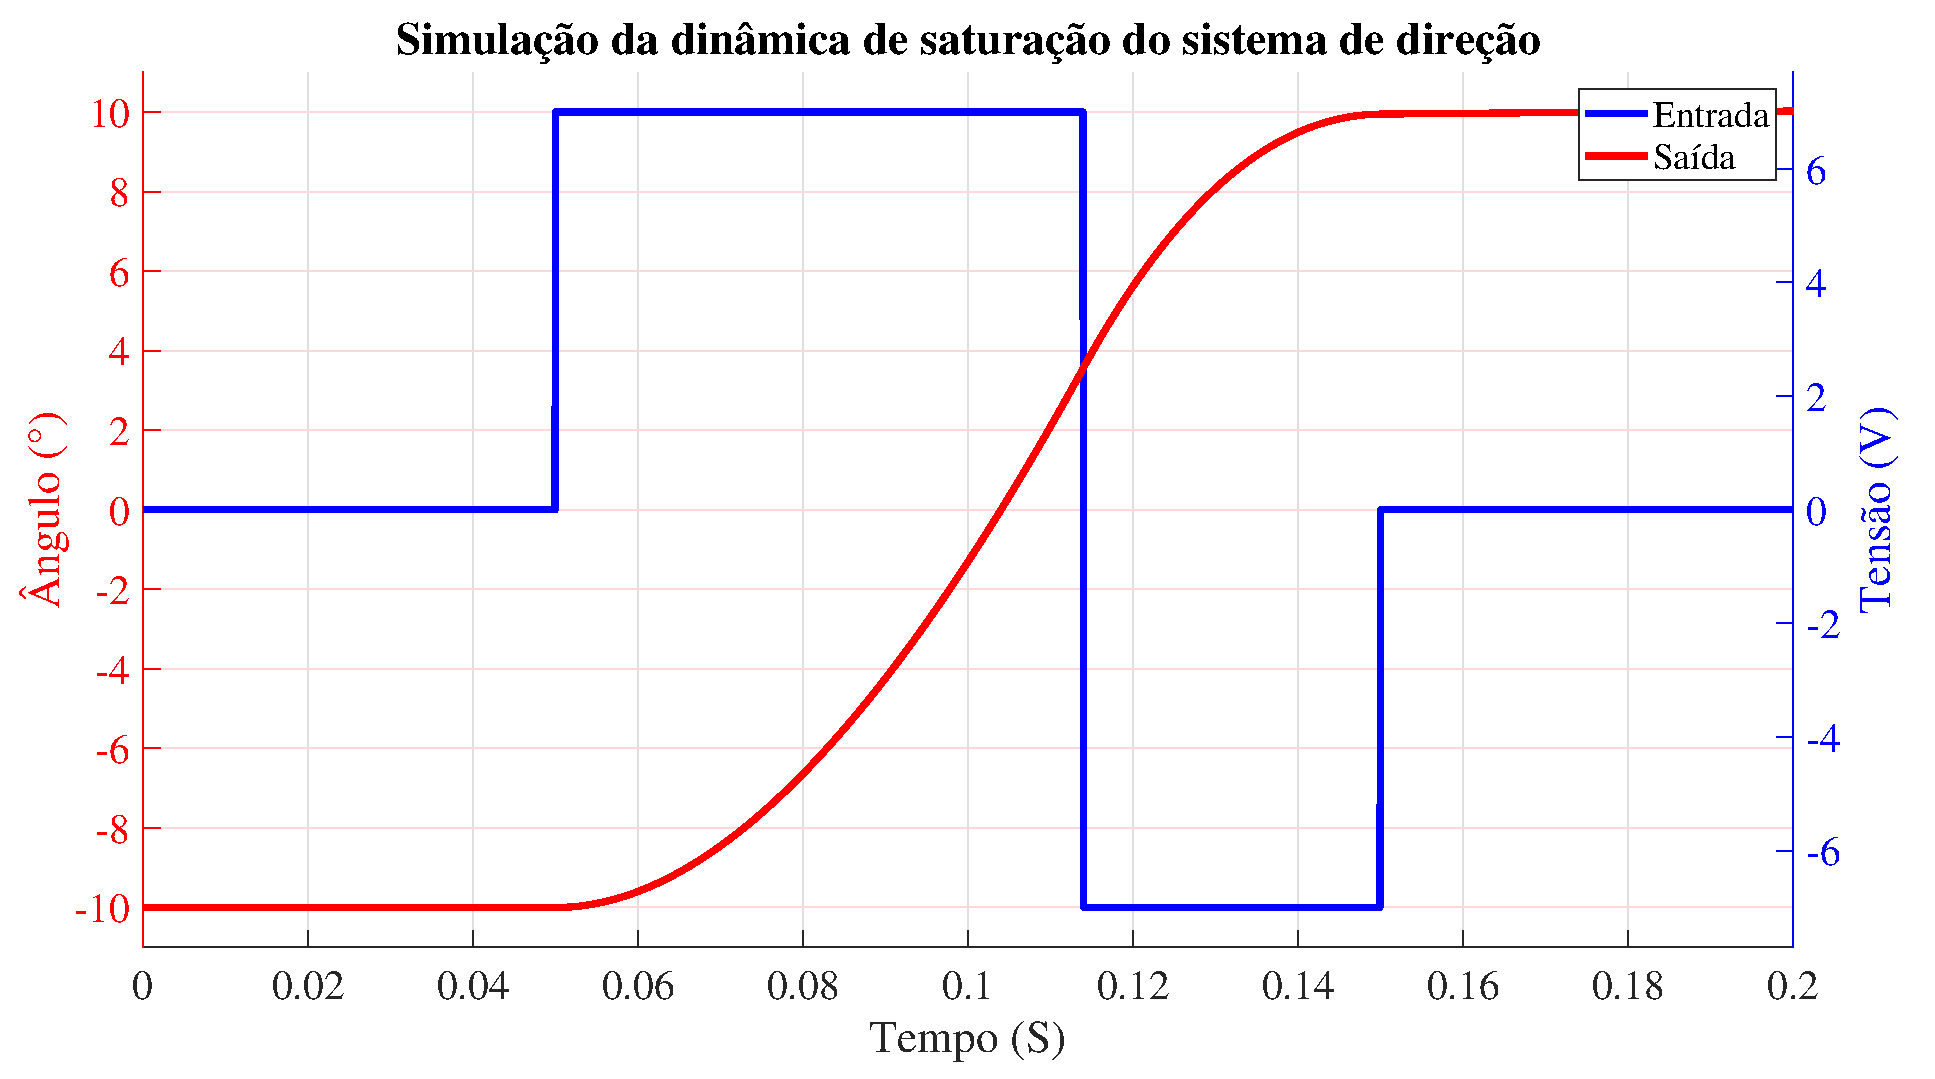
\includegraphics[width=15cm]{Imagens/cap4/sis_direcao/simusat_direcao.eps}
                \caption{Subsistemas da planta de controle}
                \label{subsistemas}
            \end{figure}
            
        \subsection{Síntese do Controlador}
	
	
	%%%%%%%%%%%%%%%%%%%%%%%%%%%%%%%%%%%%%%%%%%%%%%%%%%%%%%%%%%%%
	\section{Sistema de Direção - Controle do angulo de esterço}
	
	    A estratégia para realizar a síntese direta do controlador do ângulo de esterço, $C_d(s)$,  será de anular um polo da planta com um zero do controlador.
	    
	    Podemos rearranjar a equação \ref{eq:pdf} para se tornar
	    
	    \begin{equation}
	        P_{DF}(s) = (K_p + K_d f) \frac{s + \frac{K_p f}{(K_p + K_d f}}{s + f} = C_d(s)
	    \end{equation}
	    
	    Fazendo
	    
	    \begin{equation}
	        \frac{K_p f}{K_p + K_d f} = c_4
	    \end{equation}
	    
	    iremos posicionar o zero do controlador no polo $c_4$, o qual irão se anular.
	    
	    Logo o ramo de malha aberta do sistema de direção, $M_{ad}(s)$, se torna:
	    
	    \begin{equation}
	        M_{ad}(s) = C_d(s) G(s) = \frac{c_3}{s(s+c_4)}  (K_p + K_d f) \frac{s + c_4}{s + f} = \frac{c_3(K_p + K_d f)}{s(s+f)}
	    \end{equation}
	    
	    E e ramo de malha fechada do sistema de direção, $M_{fd}$, se torna:
	    
	    \begin{equation}
	        M_{fd}(s) = \frac{M_{ad}(s)}{1+M_{ad}(s)} = \frac{c_3 (K_p + K_d f)}{s^2 + f s + c_3(K_p + K_d f)}
	    \end{equation}
	    
	    Supondo que o sistema de malha fechado desejado, $D(s)$, seja um sistema de segunda ordem com ganho unitário, temos
	    
	    \begin{equation}
	        D(s) = \frac{\omega_n^2}{s^2 + 2 \zeta \omega_n s + \omega_n^2}
	    \end{equation}
	    
	    Igualando $D(s) = M_{fd}$ temos
	    
	    \begin{equation}
	        \frac{c_3 (K_p + K_d f)}{s^2 + f s + c_3(K_p + K_d f)} = \frac{\omega_n^2}{s^2 + 2 \zeta \omega_n s + \omega_n^2}
	    \end{equation}
	    
	    Que implica que
	    
	    \begin{equation}
	        \left\{
	        \begin{array}{cc}
    	        \omega_n^2 = c_3(K_p + K_d f)  \\
    	        c_4 = \frac{K_p f}{K_p + K_d f} \\
    	        f = 2 \zeta \omega_n
	        \end{array}\right
	    \end{equation}
	    
	    Por fim, isolando $K_p$, $K_d$ e $f$ o sistema é possível ao seguinte sistema
	    
	    \begin{equation}
	        \left\{
	        \begin{array}{cc}
    	        K_p = \frac{\omega_n^2 c_4}{2 \zeta c_3}\\
    	        K_d = \frac{2 \zeta \omega_n - c_4}{4 \zeta^2 c_3}\\
    	        f = 2 \zeta \omega_n 
	        \end{array}\right
	    \end{equation}
	    
	    \subsection{Dinâmica de Saturação}
	    
	        \begin{figure}[h]
                \centering
                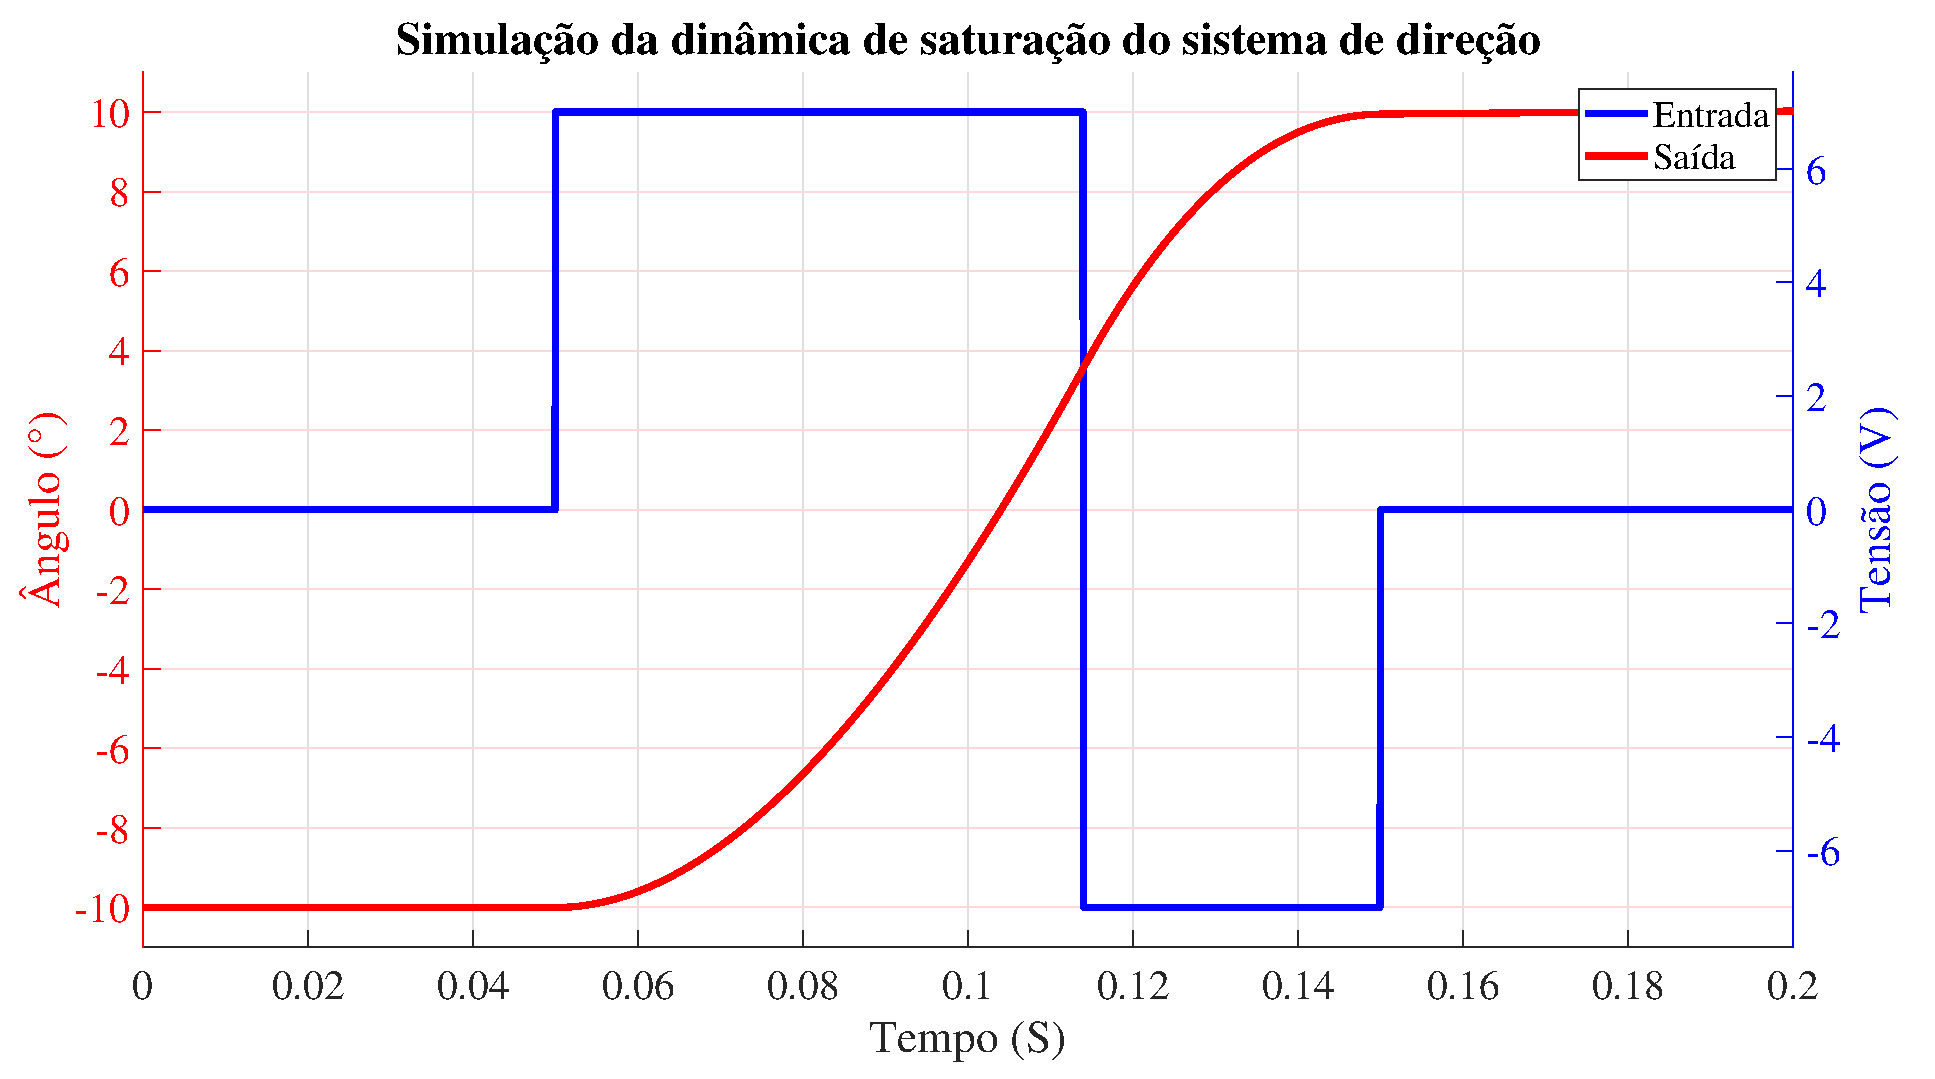
\includegraphics[width=15cm]{Imagens/cap4/sis_direcao/simusat_direcao.eps}
                \caption{Subsistemas da planta de controle}
                \label{subsistemas}
            \end{figure}
            
        \subsection{Síntese do Controlador}
        
        
        
        
	%%%%%%%%%%%%%%%%%%%%%%%%%%%%%%%%%%%%%%%%%%%%%%%%%%%%%%%%%%%%%%%55
	\section{Sistema de Equilíbrio - Controle do pendulo invertido}
	    
	    O sistema de inclinação, $G(s)$, está em série com o sistema de direção em malha fechada, 
	    \begin{equation}
	        G(s) = \frac{ \frac{v d_c}{h d_e} s + \frac{v^2}{d_e h} }{ s^2 - \frac{g}{h} }
	    \end{equation}
	    
	    
	\section{Resultados}
	
	    \subsection{Sistema de Controle de Velocidade}
	    \subsection{Sistema de Controle de direção}
	    \subsection{Sistema de Controle de Inclinação}
	    